%% ****** Start of file apstemplate.tex ****** %
%%
%%
%%   This file is part of the APS files in the REVTeX 4 distribution.
%%   Version 4.1r of REVTeX, August 2010
%%
%%
%%   Copyright (c) 2001, 2009, 2010 The American Physical Society.
%%
%%   See the REVTeX 4 README file for restrictions and more information.
%%
%
% This is a template for producing manuscripts for use with REVTEX 4.0
% Copy this file to another name and then work on that file.
% That way, you always have this original template file to use.
%
% Group addresses by affiliation; use superscriptaddress for long
% author lists, or if there are many overlapping affiliations.
% For Phys. Rev. appearance, change preprint to twocolumn.
% Choose pra, prb, prc, prd, pre, prl, prstab, prstper, or rmp for journal
%  Add 'draft' option to mark overfull boxes with black boxes
%  Add 'showpacs' option to make PACS codes appear
%  Add 'showkeys' option to make keywords appear
\documentclass[aps,prl,twocolumn,superscriptaddress]{revtex4-1}
%\documentclass[aps,prl,preprint,superscriptaddress]{revtex4-1}
%\documentclass[aps,prl,reprint,groupedaddress]{revtex4-1}

% You should use BibTeX and apsrev.bst for references
% Choosing a journal automatically selects the correct APS
% BibTeX style file (bst file), so only uncomment the line
% below if necessary.
\bibliographystyle{apsrev4-1}
%\usepackage{cite}

%\usepackage[english]{babel}
%\usepackage[utf8]{inputenc}
\usepackage{amsmath}
\usepackage{graphicx}
\usepackage{amsfonts}
%\usepackage[colorinlistoftodos]{todonotes}


\usepackage{graphicx}
\usepackage{caption}
\usepackage{subcaption}
\newcommand{\vcrm}[1]{\mathbf{#1}}
\newcommand{\hvcrm}[1]{\mathbf{\hat{#1}}}
\newcommand{\vc}[1]{\boldsymbol{#1}}
\newcommand{\hvc}[1]{\boldsymbol{\hat{#1}}}

\newcommand{\ssa}[0]{\sin{\alpha}}
\newcommand{\cca}[0]{\cos{\alpha}}
\newcommand{\ssb}[0]{\sin{\beta}}
\newcommand{\ccb}[0]{\cos{\beta}}
\newcommand{\ssc}[0]{\sin{\gamma}}
\newcommand{\ccc}[0]{\cos{\gamma}}
\newcommand{\sst}[0]{\sin{\theta}}
\newcommand{\cct}[0]{\cos{\theta}}
\newcommand{\ssp}[0]{\sin{\phi}}
\newcommand{\ccp}[0]{\cos{\phi}}

\newcommand{\dd}{\mathrm{d}}
\newcommand{\ee}{\mathrm{e}}
\newcommand{\ii}{\mathrm{i}}
\newcommand{\kk}{\mathrm{k}_B}

\newcommand{\vm}{\vc{\mu}}
\newcommand{\vn}{\hvcrm{n}}
\newcommand{\vB}{\vcrm{B}}
\newcommand{\vz}{\hvcrm{z}}


\begin{document}

% Use the \preprint command to place your local institutional report
% number in the upper righthand corner of the title page in preprint mode.
% Multiple \preprint commands are allowed.
% Use the 'preprintnumbers' class option to override journal defaults
% to display numbers if necessary
%\preprint{}

%Title of paper
\title{Entropic orientational bistability in a magnetically confined colloidal gyroscope}

% repeat the \author .. \affiliation  etc. as needed
% \email, \thanks, \homepage, \altaffiliation all apply to the current
% author. Explanatory text should go in the []'s, actual e-mail
% address or url should go in the {}'s for \email and \homepage.
% Please use the appropriate macro foreach each type of information

% \affiliation command applies to all authors since the last
% \affiliation command. The \affiliation command should follow the
% other information
% \affiliation can be followed by \email, \homepage, \thanks as well.
\author{Yongxiang Gao}
\affiliation{Department of Chemistry, Physical and Theoretical Chemistry Laboratory, University of Oxford}
\author{Andrew Kaan Balin}
\affiliation{The Sir Rudolf Peierls Centre for Theoretical Physics, University of Oxford}
\author{Roel P.A.\ Dullens}
\affiliation{Department of Chemistry, Physical and Theoretical Chemistry Laboratory, University of Oxford}
\author{Julia M.\ Yeomans}
\affiliation{The Sir Rudolf Peierls Centre for Theoretical Physics, University of Oxford}
\author{D.G.A.L.\ Aarts}
\affiliation{Department of Chemistry, Physical and Theoretical Chemistry Laboratory, University of Oxford}
%\email[]{Your e-mail address}
%\homepage[]{Your web page}
%\thanks{}
%\altaffiliation{}


%Collaboration name if desired (requires use of superscriptaddress
%option in \documentclass). \noaffiliation is required (may also be
%used with the \author command).
%\collaboration can be followed by \email, \homepage, \thanks as well.
%\collaboration{}
%\noaffiliation

\date{\today}

\begin{abstract}
We report the novel orientational behaviour of a colloidal ferromagnetic rod in a viscous medium in the presence of an external magnetic field. At equilibrium, the rod tends to lie horizontally in the plane and undergoes azimuthal thermal reorientation, while gravity suppresses large thermal deviations in inclination. A static external magnetic field acts to trap the rod, confining its azimuthal angle to maximise alignment of the magnetic moment with the field. However, we observe a significant emergence of a tendency for the rod to reorient vertically despite a corresponding increase in total energy of $\sim 4\ \kk T$. We show that this can be explained theoretically as an entropic effect, and derive analytically the Boltzmann distribution across rod orientations which shows a 2 order of magnitude increase in the probability for a rod to be found in a vertical state when trapped in a static magnetic field. We study the dynamic behaviour of the rods when driven by a rotating magnetic field and observe three distinct regimes of alignment and rod rotation. We hypothesise that these regimes arise from the anisotropic friction of the rod and employ a minimal-model Langevin simulation with no free parameters to corroborate this theory with the experimental data and explore the phase space of the system.
\end{abstract}

% insert suggested PACS numbers in braces on next line
\pacs{}
% insert suggested keywords - APS authors don't need to do this
%\keywords{}

%\maketitle must follow title, authors, abstract, \pacs, and \keywords
\maketitle

%%%%%%%%%%%%%%%%%%%%%%%%%%%%%%%%%%%%%%%%%%%%%%%%%%%%%%%%%%%%%%%%%%%%
%
%
%
%
%					I N T R O D U C T I O N
%
%
%
%%%%%%%%%%%%%%%%%%%%%%%%%%%%%%%%%%%%%%%%%%%%%%%%%%%%%%%%%%%%%%%%%%%%
%\section{Introduction}

Microscopic devices controlled or actuated by external fields ---be it magnetic, electronic or gravitational--- have a great potential to find applications in emerging nanotechnologies. It has been suggested that novel self-folding nanowires which respond to magnetic fields can be implemented in minimally invasive surgery \cite{Xi2013,Solovev2012}. Other utilities for actuated microscopic devices include the pumping or mixing of fluids, self-propulsion and active transport of colloids. However, there are two great challenges with present themselves at these length scales. Inertia, which scales with volume, tends to become vanishingly small with respect to other forces such as drag acting on a small object. Hence, dynamics are governed by the low-Reynolds number Stokes' equations where, due to time-reversibility, self-propulsion becomes a difficult task \emph{[cite?]}. 

Nanorods are a class of well studied colloidal particles characterised by an elongated shape (e.g.\ cylindrical or ellipsoidal) and a diameter of less than $1\ \mu$m. \emph{[Review here literature pertaining to actuated nanorods, magnetic or otherwise. Talk about applications e.g.\ microsurgery]}

%\section{Equilibrium}
In this letter, we demonstrate unexpected equilibrium behaviour in a ferromagnetic rod under the influence of an external magnetic field. The distribution over polar angles reveals a bistability where both flat and vertical orientations of the rod are favoured despite the latter gaining $\sim 4 \kk T$ in gravitational potential energy at no apparent reduction in stored magnetic field energy. A theoretical analysis reveals the entropic nature of this effect and predicts how the bistability may be tuned by controlling the field strength and temperature.


\begin{figure}
	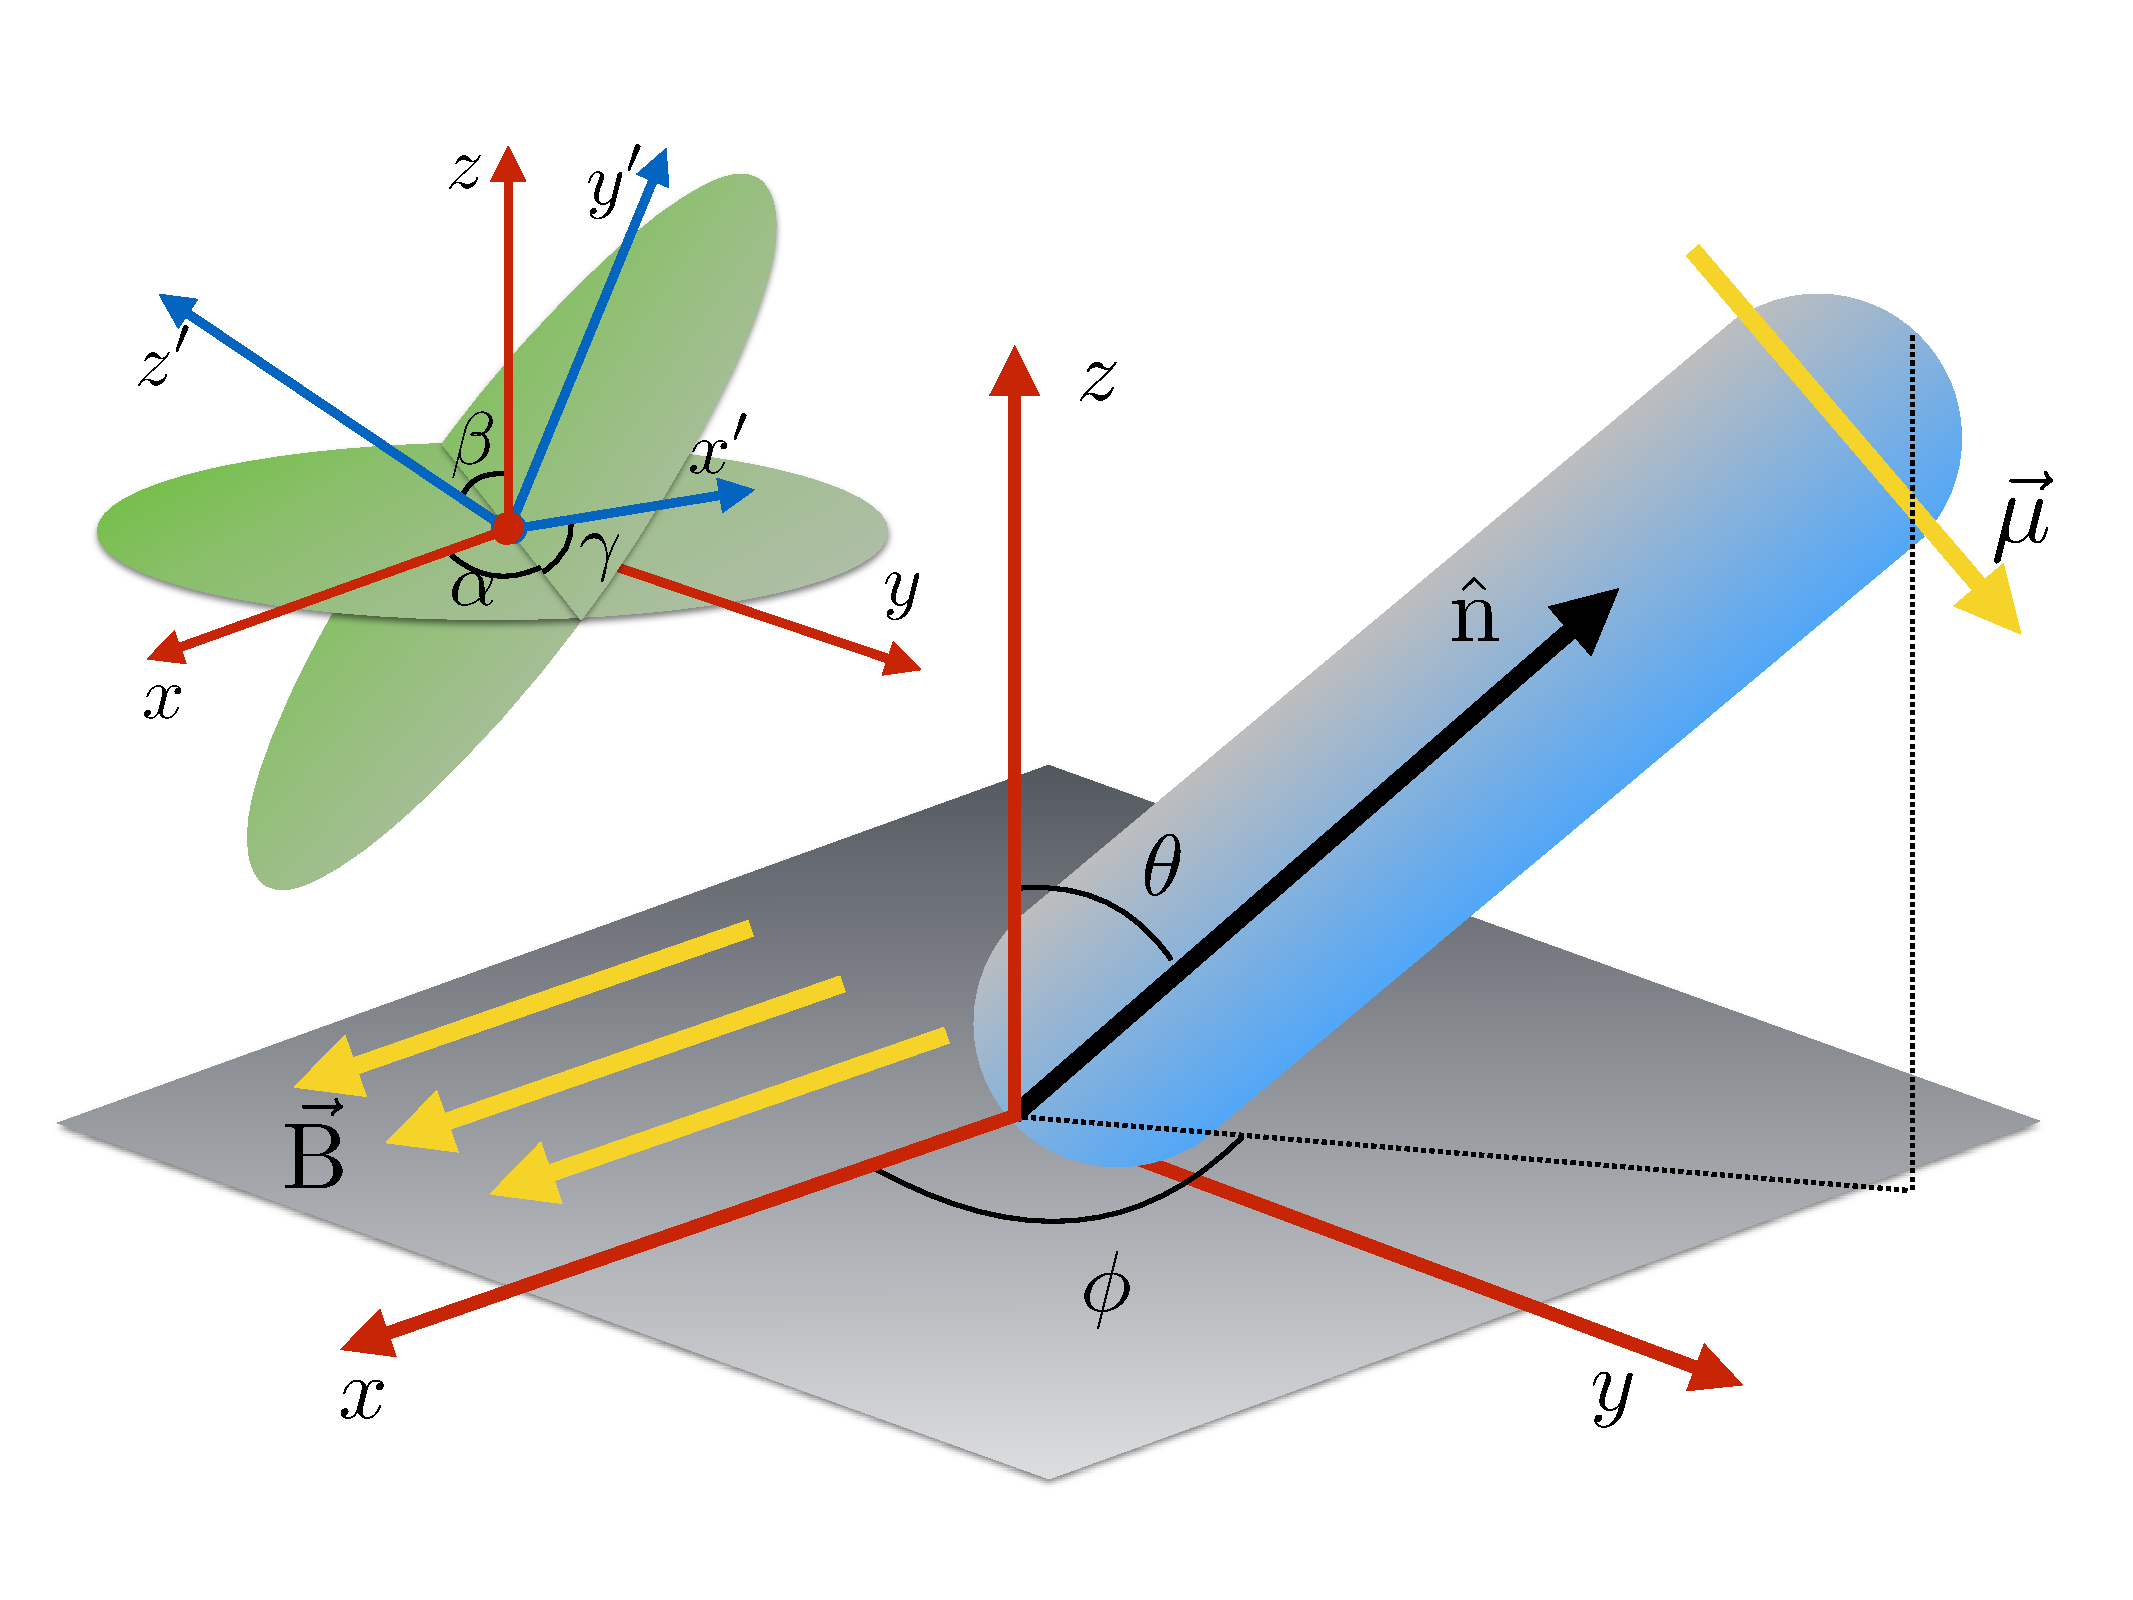
\includegraphics[width=0.98\columnwidth]{figs/geometry.pdf}
	\caption{\footnotesize Geometry and notation used throughout. A rod's shape is modelled as a cylinder of length $l$ capped by two hemispheres of diameter $d$ giving it a total length of $L=l+2d$. The orientation of the rod, $\hvcrm{n}$ is defined as the unit vector pointing along the long axis of the rod in the $+$ve $z$-direction. This makes an angle $\theta$ with the $z$-axis and its projection in the $xy$-plane subtends an angle $\phi$ with the $x$-axis. A perpendicular permanent magnetic moment $\vc{\mu}$ is embedded in one of the caps and rotates rigidly with the rod. An external magnetic field $\vcrm{B}$ is applied in the $x$-direction and interacts with $\vc{\mu}$, while a gravitational force $m^*l\cos\theta\vcrm{g}/2$ in the $-$ve $z$-direction interacts with $\hvcrm{n}$. Inset: Euler angles are useful for describing the fixed-body rotation of the rod, where $\hvcrm{n}=\hvcrm{z}'$, $\vc{\mu}=\mu\hvcrm{x}'$, $\beta=\theta$, and $\alpha=\phi+\frac{\pi}{2}$.\label{fig:geometry}}
\end{figure}

\emph{[Synthesis, assay, microscopy to be added around here]}. Figure \ref{fig:geometry} illustrates the shape of a typical rod synthesised using this process, as well as the coordinate system we use to describe its orientation. The rod closely resembles a hemispherically capped cylinder, with total length measured to be $L=3.5\pm0.1 \mu$m and diameter $d = 0.65\pm0.01 \mu$m \emph{[What are the real errors on these?]}. The long axis of the cylinder is spanned by $\hvcrm{n}$ which makes an angle $\theta$ with the $z$-axis, and an angle $\phi$ in the $xy$-plane. One cap of the rod has embedded in it a permanent magnetic moment $\vc{\mu}$ that is perpendicular to $\hvcrm{n}$ and requires a third angle, $\gamma$, to parameterise its direction in the cross-sectional plane of the rod. If we take the fixed-body coordinates of the rod, $(x',y',z')$, then $\hvcrm{n}$ lies along the $z'$-axis, $\vc{\mu}$ lies along the $x'$-axis, and the conventional Euler angles $(\alpha=\phi+\pi/2, \beta=\theta, \gamma)$ describe the rotation of the rod-frame relative to the lab-frame. 

Due to its large density relative to water, ($\rho_r = 1.9 \cdot 10^3$ kgm$^{-3}$) a rod undergoes fast sedimentation on the coverslip of the microscope slide and will naturally lie horizontally in the plane ($\theta=\pi/2$) whilst undergoing rotational Brownian motion in $\phi$. Such motion in $\theta$ is heavily suppressed by gravity. In the presence of an in-plane magnetic field $\vcrm{B}=B\hvcrm{x}$, the rod aligns with the $y$-axis (in either $+$ve or $-$ve direction) as $\vc{\mu}$ aligns with $\vcrm{B}$. We make use of the equipartition theorem $\langle -\vc{\mu}\cdot\vcrm{B}\rangle = \frac{1}{2}\mu B \langle \Delta\phi^2 \rangle = \frac{1}{2}\kk T$ to calculate the strength of the moment $\mu$ by measuring the fluctuations $\Delta\phi=\phi-\phi_0$ at varying field strengths at room temperature. The assumption we make here is that for small deviations from $\phi_0$, the rod experiences an approximately \emph{Hookean} torque: $\tau = -k_\phi \sin{\Delta\phi}\approx-k_\phi\Delta\phi$, which gives rise to the quadratic energy $U_B=-\frac{1}{2}k_\phi \Delta\phi^2$ with spring constant given by $k_\phi=\mu B$. Figure \ref{fig:trap} shows that the spread of $\Delta\phi$ decreases for larger $B$, and does so in a manner whereby $\mu(B)$ remains constant across the full range of fields applied. With these results we were able to measure the strength of the moment of each rod. Typically, we found their strength to be approximately $ 2 \ \kk T$Ga$^{-1}$ \emph{[error?]} at room temperature.

The external field $\vcrm{B}$ interacts with $\vc{\mu}$ via the torque $\vc{\tau}_B = \vc{\mu}\times\vcrm{B}$ while the gravitational force $\vcrm{g}=-m^*g\hvcrm{z}$ interacts with $\hvcrm{n}$ by exerting a torque $\vc{\tau}_g=\frac{l}{2}\vcrm{g}\times\hvcrm{n}$. The gravitational potential gained by lifting the rod vertically is $\frac{m^* g l}{2}$, where $m^* = V(\rho_r - \rho_w)$ is the effective mass of the rod in water and $g$ is the gravitational acceleration. At room temperature, this value is approximately $4\ \kk  T$, which explains the rod's tendency to lie flat, as thermal excitations are not enough to reorient it vertically. 

However, when trapped in a magnetic field, we measured an increased tendency for the elevation of a rod to climb to a vertical orientation. This is in contrast to the gravitational suppression of such motion when no external field was applied. \emph{[Reference movie in SI?]} Interestingly, this behaviour occurs is in spite of the fact that such a trajectory sees the rod evolving from a global energy minimum to a state with an energy $\sim 4\ \kk T$ greater. We ruled out the hypothesis that there might be a repulsive interaction between the surface and the magnetic moment after noticing that the magnetic cap ended up on the top or bottom of the rod with equal probability. \emph{[Can we confirm that this is true?]}


\begin{figure}
	\begin{subfigure}[b]{0.95\columnwidth}
    	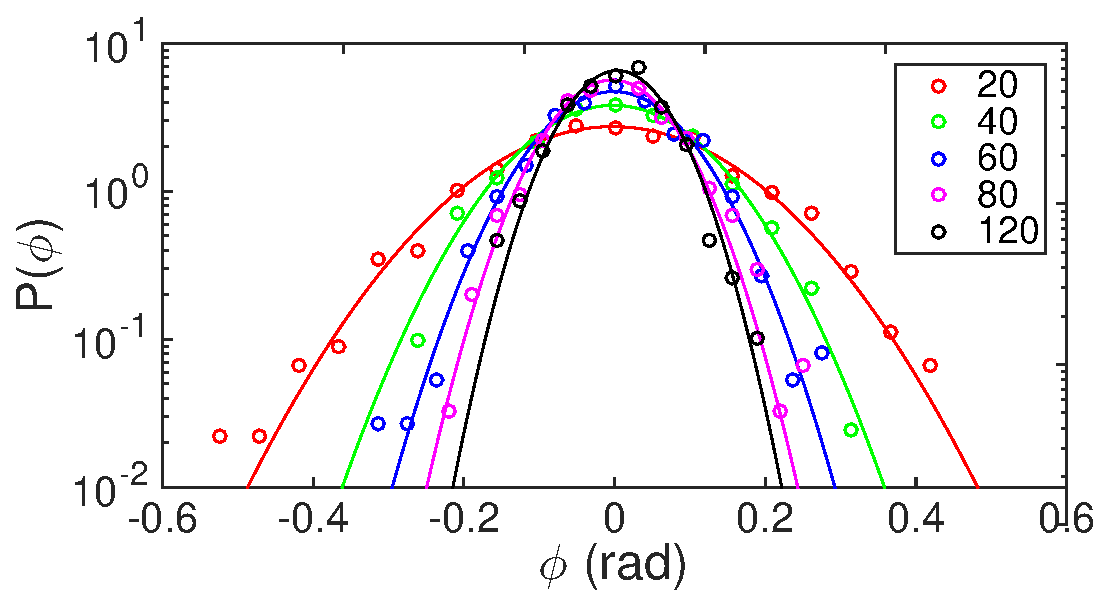
\includegraphics[width=\textwidth]{figs/Figure2a.eps}
    	\caption{}
    \end{subfigure}
    \begin{subfigure}[b]{0.95\columnwidth}
    	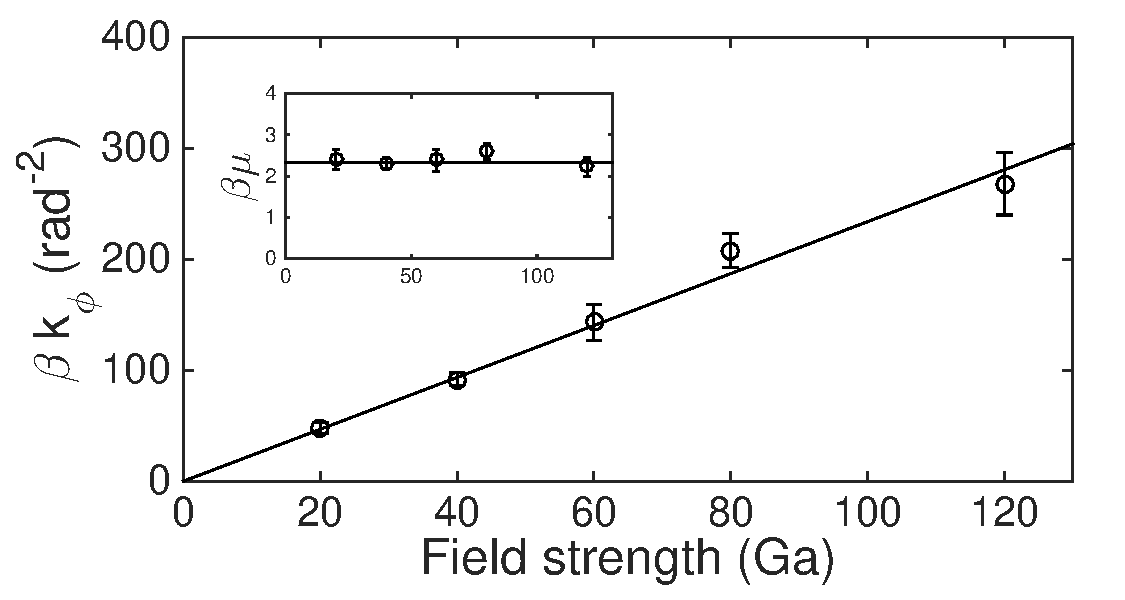
\includegraphics[width=\textwidth]{figs/Figure2b.eps}
    	\caption{}
    \end{subfigure}
    \caption{\footnotesize (a) Probability distribution of the azimuthal angle of deviation $\phi$ of the rod from alignment with a static magnetic field. The data appear to be distributed normally with a spread $\langle \phi^2 \rangle$ obtainable by applying a Gaussian fit. (b) The equipartition theorem states $\frac{1}{2} k_\phi \langle \phi^2 \rangle = \frac{1}{2}\kk T$ where $k_\phi =\mu B$ is the stiffness of the torsional trap. We make use of this to show that $\kk T / \langle \phi^2 \rangle $ increases linearly with $B$, in other words, $\mu$ remains constant across the range of field strengths used. Inset: We estimate the magnetic moment to have a permanent magnitude $\mu = 2.3\pm0.2 \ \kk T$Ga$^{-1}$.\label{fig:trap}}
	\label{fig:moment}
\end{figure}

To explain this effect, we consider the equilibrium thermodynamics of the rod. Each state of the rod $(\vm,\vn)$ can be described in terms of the angles $(\phi, \theta, \gamma)$ which relate its fixed-body frame to the laboratory frame. In the Appendix, we show that the total energy $U = -\vm \cdot\vB + \frac{l}{2} \vn \cdot \vcrm{g}$ can be expressed in terms of the angles as:

\begin{equation}
U = -\mu B (\ccc\ssp + \cct\ccp\ssc) + \frac{m^*gl}{2} \cct.
\end{equation}

Assuming that the states are Boltzmann distributed gives us:

\begin{eqnarray}
P(\phi, \theta, \gamma)  =  \frac{1}{Z} \ee^{ -U(\phi, \theta, \gamma)/\kk T }, \\
Z  =  \int_0^{\frac{\pi}{2}} \sst\ \dd\theta \iint_{-\pi}^{\pi}\ \dd\phi\ \dd\gamma \ \ee^{ -U(\phi, \theta, \gamma)/\kk T }.
\end{eqnarray}

To find the marginal distribution $P(\theta)$, we integrate out the $\phi$ and $\gamma$ dependence:

\begin{eqnarray}
P(\theta)  & = & \frac{\ee^{-a\cos\theta}}{Z} \iint_{-\pi}^{\pi} \dd\phi \dd\gamma \  \ee^{b(\ccc\ssp + \cct\ccp\ssc) }.
\end{eqnarray}

Here we have reduced the relative strength of the gravitational torque: $a=m^*gl/2 \kk T$ and magnetic torque: $b=\mu B/\kk T$. The integral over $\gamma$ may be carried out explicitly, giving:

\begin{eqnarray}
P(\theta)  & = & \frac{\ee^{-a\cos\theta}}{Z} \int_{-\pi}^{\pi}\dd\phi\ I_0\Big( b\sqrt{1-\cos^2\phi\sin^2\theta} \Big)
\end{eqnarray}where $I_n(x)$ is the modified Bessel function of the first kind. In Fig.\ \ref{fig:data} we have plotted this function for varying field strengths, $b$, against data obtained by measuring the projected length of a single-rod in the $xy$-plane of the image. Using the projected length, $\lambda$, we approximated the angle using the formula $\sin\theta = \lambda - \delta(\theta)$ \emph{[This might not be what Yongxiang used, in which case replace this section]}. This was to compensate for the fact that the top end of the rod would shift out of focus adding to the apparent projected length an amount $\delta(\theta)$. We assumed that $\delta$ was linear in $\cos\theta$ (the height of the rod endpoint), with $\delta(\pi/2)=0$ when in focus, and $\delta(0)=\delta_0$ found by manual calibration. As we are mainly interested with behaviour near $\theta=0,\pi/2$, the validity of the linear approximation of $\delta(\theta)$ for intermediate angles is not critical. The  Data were taken for $[X]$ s at a sample rate of $[Y]$ Hz.

Both the data and the theory show not just an increase in $P(\theta)$ for small $\theta$, but in fact the emergence of a peak at $\theta=0$. This and the $\theta=\pi/2$ global maximum are separated by a trough in the probability distribution, which in the canonical ensemble represents an entropic barrier. Thus, the resulting bistability is an entropic effect alone, controlled by the relative magnitudes of $\mu B$, $m^*gl/2$ and $\kk T$ and thus tunable through the externally applied field strength and temperature. \emph{[I'm currently trying to do some work on how the bistability may be tuned by these]}


\emph{[Section about dynamics to come]}


\begin{figure}
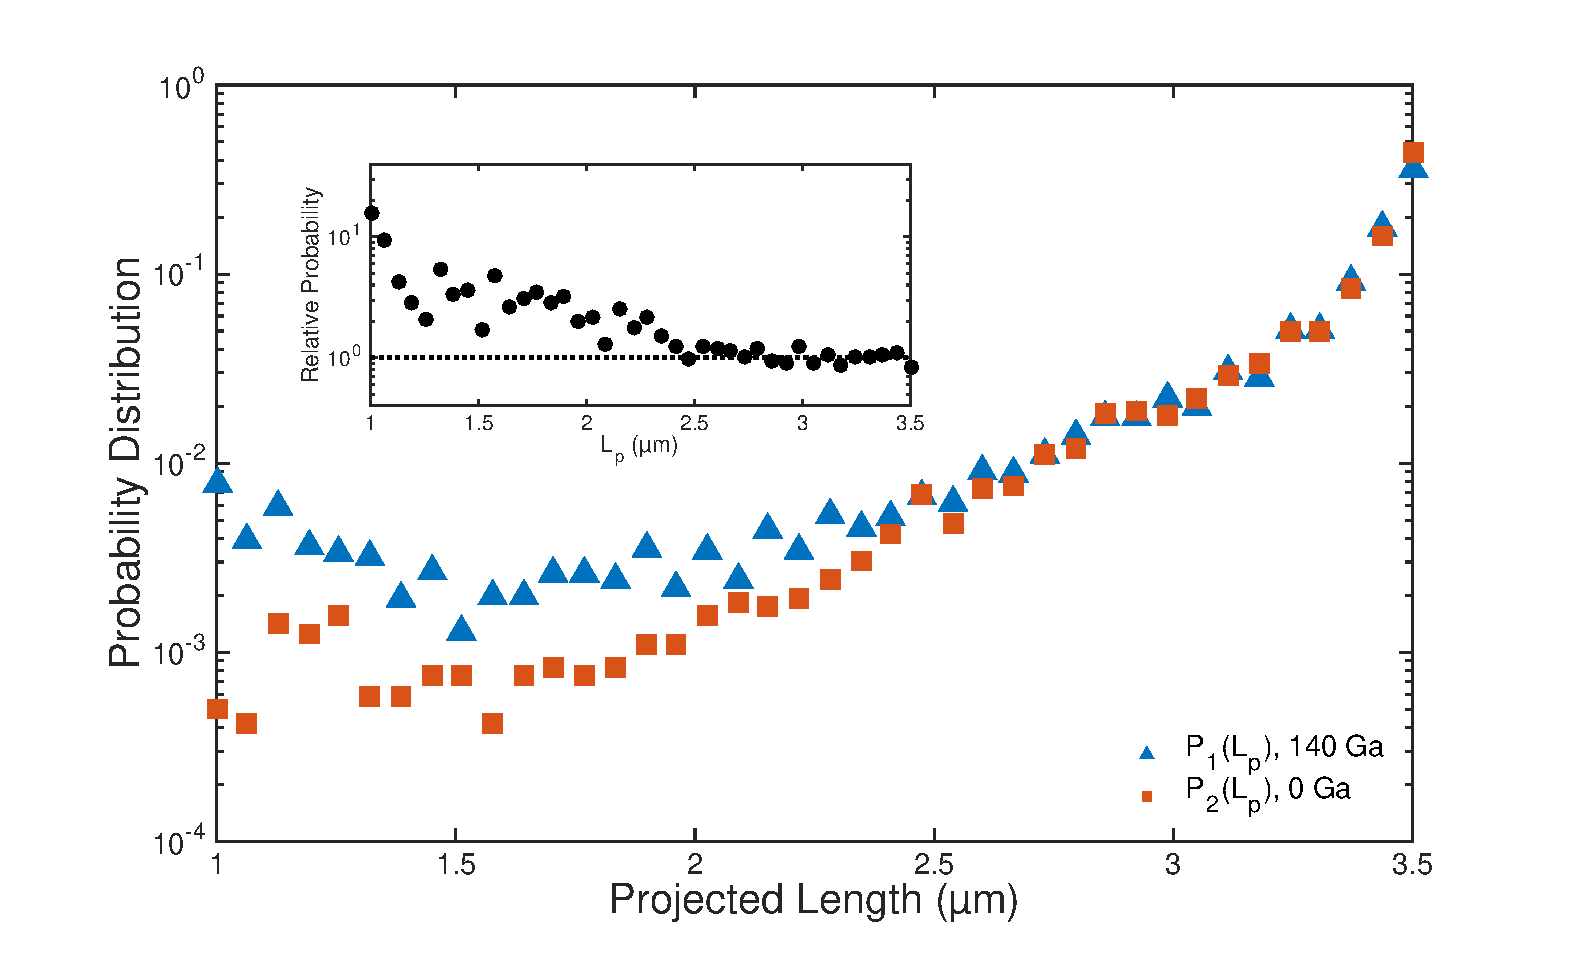
\includegraphics[width=0.95\columnwidth]{figs/Figure3.eps}
\caption{\footnotesize At equilibrium, the presence of a magnetic field has the effect of altering the distribution over polar angle $\theta$ resulting in the emergence of a peak at $\theta=0$. The vertical and horizontal alignments are thus bistable, separated by an entropic barrier. \label{fig:data} \emph{[Will write more here once we have properly converted the data to distribution over theta.]}}
\end{figure}

\begin{figure}
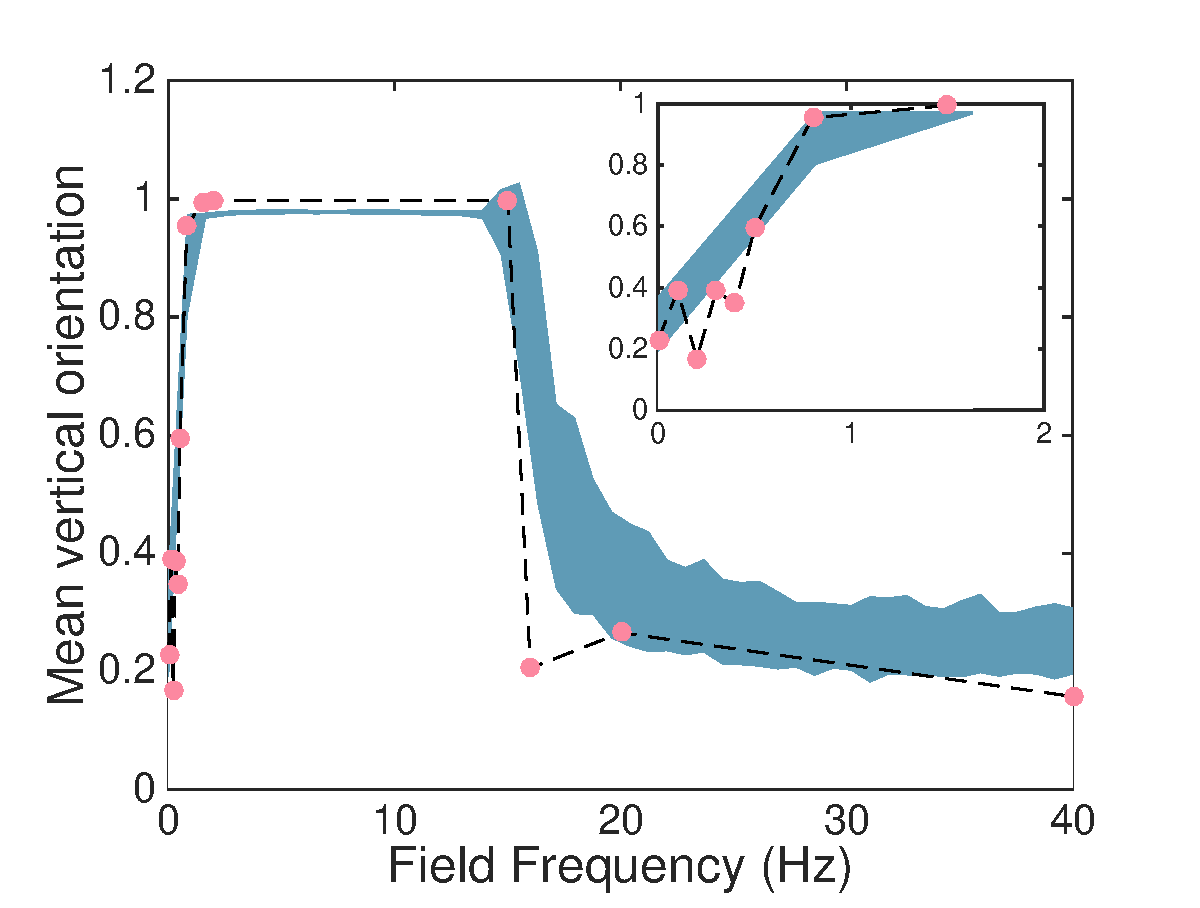
\includegraphics[width=0.95\columnwidth]{figs/Figure_n.eps}
    	\caption{\footnotesize The time-averaged alignment of rod with $z$-axis, $\langle \hvcrm{n}\cdot\hvcrm{z}\rangle$, for varying external field frequency at $B=50$ Ga. The shaded region represents the mean and standard deviation of results from 100 realisations of a Langevin simulation with no variable parameters, and shows good agreement with the data. This provides evidence to the hypothesis that the frictional anisotropy of the rod gives rise to two threshold frequencies, between which only vertical synchronous rotation of the rod is stable. Inset: Low frequency detail of main figure.}
\end{figure}


%For a rod pivoting about one of its ends, it feels a gravitational torque $\vc{\tau}_g = \frac{m^* L}{2} \hvcrm{n}\times\vcrm{g}$, where $\vcrm{g} = -g\hvcrm{z}$ is the gravitational acceleration. In the presence of an external magnetic field, an additional torque $\vc{\tau}_B = \hvc{\mu}\times\vcrm{B}$ is felt. At $T=290$ K, the characteristic strengths of these torques are $|\vc{\tau}_g| \sim 6 \kk$T, and $|\vc{\tau}_B| \sim\ $0-250$\ \kk$T (for fields in the range of $B=\ $0-120 Ga)

%\emph{Distribution}


%\section{}
% Put \label in argument of \section for cross-referencing
%\section{\label{}}
%\subsection{}
%\subsubsection{}

% If in two-column mode, this environment will change to single-column
% format so that long equations can be displayed. Use
% sparingly.
%\begin{widetext}
% put long equation here
%\end{widetext}

% figures should be put into the text as floats.
% Use the graphics or graphicx packages (distributed with LaTeX2e)
% and the \includegraphics macro defined in those packages.
% See the LaTeX Graphics Companion by Michel Goosens, Sebastian Rahtz,
% and Frank Mittelbach for instance.
%
% Here is an example of the general form of a figure:
% Fill in the caption in the braces of the \caption{} command. Put the label
% that you will use with \ref{} command in the braces of the \label{} command.
% Use the figure* environment if the figure should span across the
% entire page. There is no need to do explicit centering.

% \begin{figure}
% \includegraphics{}%
% \caption{\label{}}
% \end{figure}

% Surround figure environment with turnpage environment for landscape
% figure
% \begin{turnpage}
% \begin{figure}
% \includegraphics{}%
% \caption{\label{}}
% \end{figure}
% \end{turnpage}

% tables should appear as floats within the text
%
% Here is an example of the general form of a table:
% Fill in the caption in the braces of the \caption{} command. Put the label
% that you will use with \ref{} command in the braces of the \label{} command.
% Insert the column specifiers (l, r, c, d, etc.) in the empty braces of the
% \begin{tabular}{} command.
% The ruledtabular enviroment adds doubled rules to table and sets a
% reasonable default table settings.
% Use the table* environment to get a full-width table in two-column
% Add \usepackage{longtable} and the longtable (or longtable*}
% environment for nicely formatted long tables. Or use the the [H]
% placement option to break a long table (with less control than 
% in longtable).
% \begin{table}%[H] add [H] placement to break table across pages
% \caption{\label{}}
% \begin{ruledtabular}
% \begin{tabular}{}
% Lines of table here ending with \\
% \end{tabular}
% \end{ruledtabular}
% \end{table}

% Surround table environment with turnpage environment for landscape
% table
% \begin{turnpage}
% \begin{table}
% \caption{\label{}}
% \begin{ruledtabular}
% \begin{tabular}{}
% \end{tabular}
% \end{ruledtabular}
% \end{table}
% \end{turnpage}

% Specify following sections are appendices. Use \appendix* if there
% only one appendix.
%\appendix
\appendix*
\section{Appendix \emph{[or SI?]}}
We wish to evaluate the energy $U = -\vm \cdot\vB + \frac{ml}{2} \vn \cdot \vcrm{g}$. It is simplest if we write down the first term in the fixed-body frame of the rod, where $\vm=(\mu,0,0)$, and the second term in the lab frame where $\vcrm{g} = (0,0,-g)$. This leaves us with the task of expressing $\vB$ in the rod frame:

\begin{equation}
\vc{\mu}\cdot\vcrm{B}  =  (\mu,0,0) \cdot \vcrm{R} \begin{pmatrix} B \\ 0 \\ 0\end{pmatrix}
\end{equation}, where $\vcrm{R}$ is the Euler rotation matrix that transforms $(x,y,z)$ to $(x',y',z')$. Only the $xx$-component is required, which gives us $\vm \cdot\vB = \mu B (\ccc\cca - \ccb\ssa\ssc)$.

By a change of variables to the previously defined azimuthal and polar angles, $\alpha\rightarrow\phi+\frac{\pi}{2}$, and $\beta\rightarrow\theta$, we get:

\begin{equation}
\vm \cdot\vB  = -\mu B (\ccc\ssp + \cct\ccp\ssc).
\end{equation}

The normal vector is expressed in the lab frame as the familiar $\vn = (\ccp\sst, \ssp\sst, \cct)$ which finally yields $\frac{ml}{2}\hvcrm{n}\cdot\vcrm{g} = -\frac{mlg}{2}\cct$.

%\section{}

% If you have acknowledgments, this puts in the proper section head.
%\begin{acknowledgments}
% put your acknowledgments here.
%\end{acknowledgments}

% Create the reference section using BibTeX:
\bibliography{refs/refs.bib}

\end{document}
%
% ****** End of file apstemplate.tex ******

